\documentclass[10pt]{article}

\usepackage[utf8]{inputenc}
\usepackage[T1]{fontenc}
\usepackage{lmodern}
\usepackage{geometry}
\geometry{margin=1in}

\usepackage{float}
\usepackage{amsmath,amssymb}
\usepackage{graphicx}
\usepackage{booktabs}
\usepackage{natbib}
\usepackage{hyperref}
\hypersetup{
    colorlinks = true,
    linkcolor  = blue,
    citecolor  = blue,
    urlcolor   = blue
}

\title{%
  \textbf{Reddit Comment Engagement Analysis}\\
  \large DATA 410/STAT 538 Final Report
}
\author{%
  \textbf{Group Members:} \\ 
  Aarav Gosalia, Aleric Govender, Jordi Capdevila Maso
}
\date{\today}


\begin{document}
\maketitle

\tableofcontents
\clearpage

\section{Introduction}

Reddit, with approximately 2 billion monthly visits \cite{statista2023}, is one of the world's most popular social media platforms, renowned for its distinctive, topic-based communities known as subreddits. \\

\noindent These subreddits function as individual forums centered around specific interests, each with its own culture, rules, and moderators. Users interact by posting content and commenting, and express approval or disapproval through upvotes and downvotes, which determine a comment’s score—a net value that reflects its reception within the community. This score can be positive, negative, or zero, serving as a useful proxy for engagement \\

\noindent In this project, we investigate the factors that drive higher engagement on Reddit comments by analyzing features such as sentiment, text characteristics, and metadata (e.g., user karma, comment hour, etc.) Our main hypothesis is to determine whether the sentiment of a Reddit comment has an effect on its popularity and if metadata features play a significant role in driving that popularity.\\

\noindent In the sections that follow, we first describe the dataset and our data collection process, then detail our exploratory data analysis which lays the foundation for the subsequent regression modeling.

%--------------------------------------------------

\subsection{Dataset Overview}
Our dataset includes subreddits that span a broad spectrum of topical focuses, user demographics, and conversational norms. For instance, r/AskReddit features open-ended Q\&A threads with a massive user base, r/datascience and r/technology focus on more technical or professional discussions, and r/FloridaMan often highlights humorous or eccentric news stories. Subreddits like r/movies and r/gaming center on entertainment and fan-driven content, whereas r/books and r/health lean toward more intellectual or personal experiences. Meanwhile, r/Showerthoughts emphasizes concise, thought-provoking ideas, and r/UnpopularOpinion showcases contrarian or debate-oriented posts. By drawing from these distinct communities, we capture a wide range of linguistic styles, engagement patterns, and discourse behaviors in our final dataset.\\

\noindent In total, our dataset contains \textbf{37,757 observations} and \textbf{16 variables}. Our primary response variable is \texttt{Comment Score}, defined as the net difference between upvotes and downvotes on a comment.

%--------------------------------------------------

\subsection{Data Collection Process}
We collected the data in real-time using the \texttt{PRAW} (Python Reddit API Wrapper) \cite{praw2024} library to ensure our dataset remained up-to-date with the latest comments. Specifically, we extracted the top posts from each subreddit, retrieved the associated comment threads, and stored all relevant metadata and text content in CSV format. This process allowed us to capture a diverse range of topics, timeframes, and user interactions across the selected subreddits. \\

\noindent The dataset consists of 16 features, categorized as:

\begin{itemize}
    \item \textbf{Continuous Variables:}
    \begin{itemize}
        \item \texttt{sentiment score} : A numerical score indicating the emotional tone of the comment, ranging from \(-1\) (very negative) to \(1\) (very positive).
        \item \texttt{comment score} : The net total of upvotes minus downvotes that a comment receives.
        \item \texttt{number of replies} : The total number of direct replies a comment receives.
        \item \texttt{text length} : The number of characters in the comment.
        \item \texttt{word count} : The number of words in the comment.
        \item \texttt{comment age (hours)} : The time (in hours) between the original post and when the comment was made.
        \item \texttt{parent score} : The comment score of the comment or post that this comment is replying to.
        \item \texttt{user karma} : A score reflecting the overall contribution and reputation of a Reddit user.
        \item \texttt{account age} : The number of days since the Reddit user created their account.
    \end{itemize}
    
    \item \textbf{Categorical Variables:}
    \begin{itemize}
        \item \texttt{subreddit name} : The name of the subreddit where the comment was posted.
        \item \texttt{comment hour} : The hour of the day (from 0 to 23) when the comment was posted.
        \item \texttt{comment day} : The day of the week (from 0 = Monday to 6 = Sunday) the comment was posted.
    \end{itemize}
    
    \item \textbf{Binary Variables:}
    \begin{itemize}
        \item \texttt{contains emoji} : 1 if the comment contains any emoji, 0 otherwise.
        \item \texttt{contains question} : 1 if the comment includes a question (e.g., contains “?” or is interrogative), 0 otherwise.
        \item \texttt{contains profanity} : 1 if the comment contains profane language, 0 otherwise.
        \item \texttt{is early comment} : 1 if the comment was posted within one hour of the original post, 0 otherwise.
    \end{itemize}
\end{itemize}

\noindent Before analysis, we performed basic data cleaning to remove deleted or bot-generated comments, which are typically automated responses posted by scripts or programs rather than real users, often used for moderation, spam, or repetitive tasks. We then applied SpaCy \cite{spacy2023} for natural language processing (NLP) tasks, such as detecting whether a comment contains a question by analyzing sentence structure. For sentiment analysis, we used the VADER (Valence Aware Dictionary and Sentiment Reasoner) tool \cite{hutto2014}, which is designed for social media text and assigns a sentiment score based on the presence of positive, negative, and neutral words. Together, these steps provided a structured, feature-rich dataset that captures both the linguistic and engagement aspects of Reddit comments.

%--------------------------------------------------

\subsection{Exploratory Data Analysis}

We begin our analysis by examining the main numeric variables in the dataset. Table~\ref{tab:summary-stats} provides basic descriptive statistics, including the minimum, first quartile (1Q), median, mean, third quartile (3Q), and maximum values. These metrics help us gauge the overall spread and central tendencies of each variable.

\begin{table}[H]
\centering
\begin{tabular}{lcccccc}
\toprule
& \textbf{Comment Score} & \textbf{Sentiment Score} & \textbf{Parent Score} & \textbf{User Karma} & \textbf{Account Age (days)} \\
\midrule
\textbf{Min}  & -768    & -0.9981 & -538    & -100     & 0    \\
\textbf{1Q}   & 1       & -0.25   & 11      & 3265     & 769  \\
\textbf{Median} & 3     & 0       & 139     & 17766    & 2137 \\
\textbf{Mean}   & 33.54 & 0.08411 & 3258    & 65993    & 2326 \\
\textbf{3Q}   & 9       & 0.4767  & 1139    & 64860    & 3787 \\
\textbf{Max}  & 22077   & 0.9995  & 60446   & 6272141  & 7041 \\
\bottomrule
\end{tabular}
\caption{Summary statistics for five key numeric variables (columns) in the dataset.}
\label{tab:summary-stats}
\end{table}

\noindent As shown in Table~\ref{tab:summary-stats}, our main response variable, \texttt{Comment Score}, exhibits a large range, from \(-768\) to \(22{,}077\). The mean is notably higher than the median, suggesting a right-skewed distribution driven by a relatively small number of very high-scoring comments. To better understand the shape of this distribution within a more typical range of values, we next present a restricted histogram of Comment Score truncated to the interval [-10, 50], which captures the bulk of observations while excluding extreme outliers.

\begin{figure}[H]
    \centering
    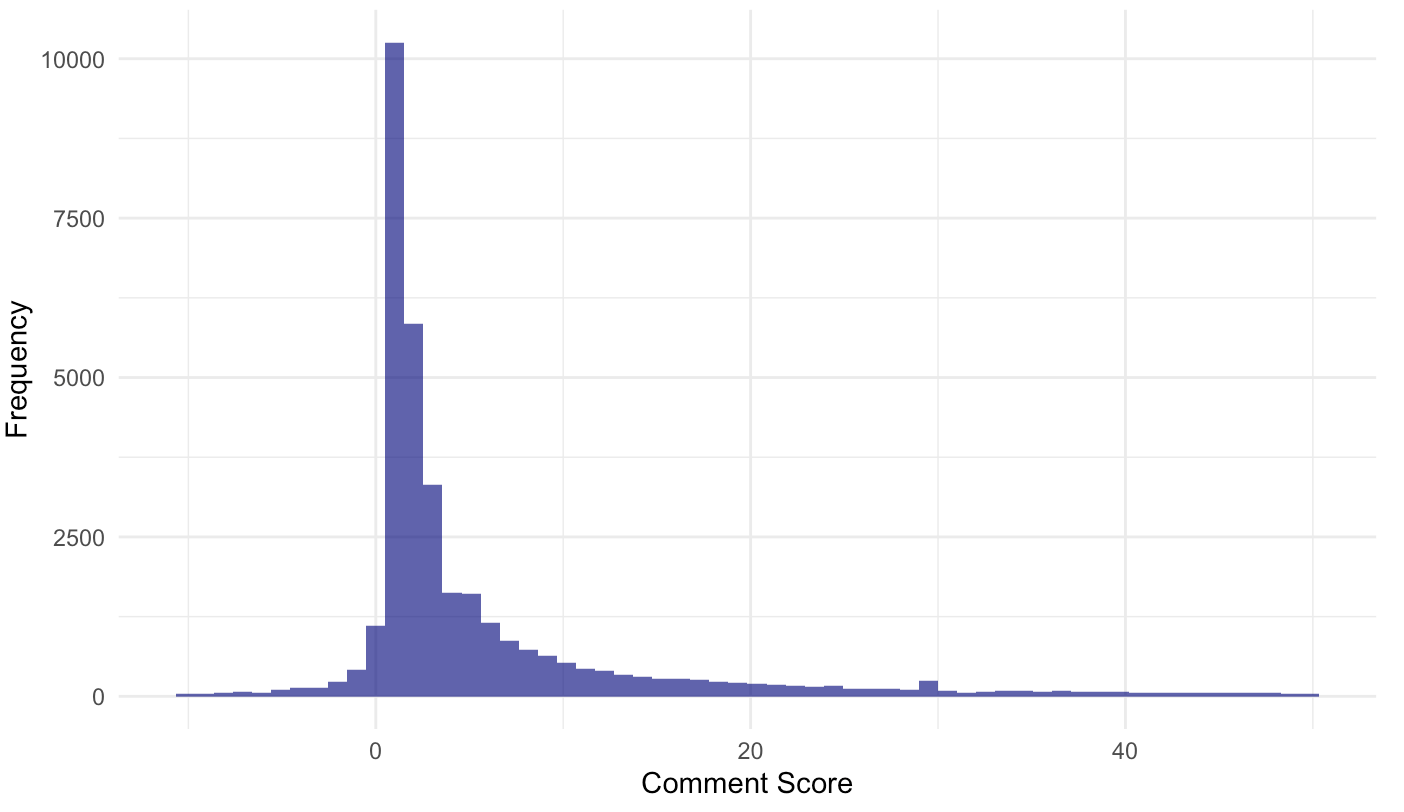
\includegraphics[width=0.8\textwidth]{pictures/score_distribution_zoomed.png}
    \caption{Truncated distribution of Comment Score restricted to values from -10 to 50.}
    \label{fig:comment-score-zoomed}
\end{figure}

\noindent As shown in Figure~\ref{fig:comment-score-zoomed}, most comment scores fall between 0 and 10, with the mode occurring around 2-3. Because the distribution spans negative, zero, and positive values, a standard log transform is not directly applicable. One alternative is the inverse hyperbolic sine (\(\operatorname{asinh}\)) transformation, which remains defined for all real numbers and behaves similarly to a log transform for large magnitudes \citep{burbidge1988, mackinnon1990}. Another option is to shift the entire distribution to be strictly nonnegative and then apply a log‐ or count‐based approach (e.g., Poisson or negative binomial) \cite{cameron1998}. In the sections that follow, we will examine both the \(\operatorname{asinh}\) method and a shifting strategy to determine which modeling framework best captures the behavior of Comment Score.

%--------------------------------------------------

\section{Regression Analysis}

\subsection{Approach 1: Inverse Hyperbolic Sine (IHS) Model}
\begin{figure}[H]
    \centering
    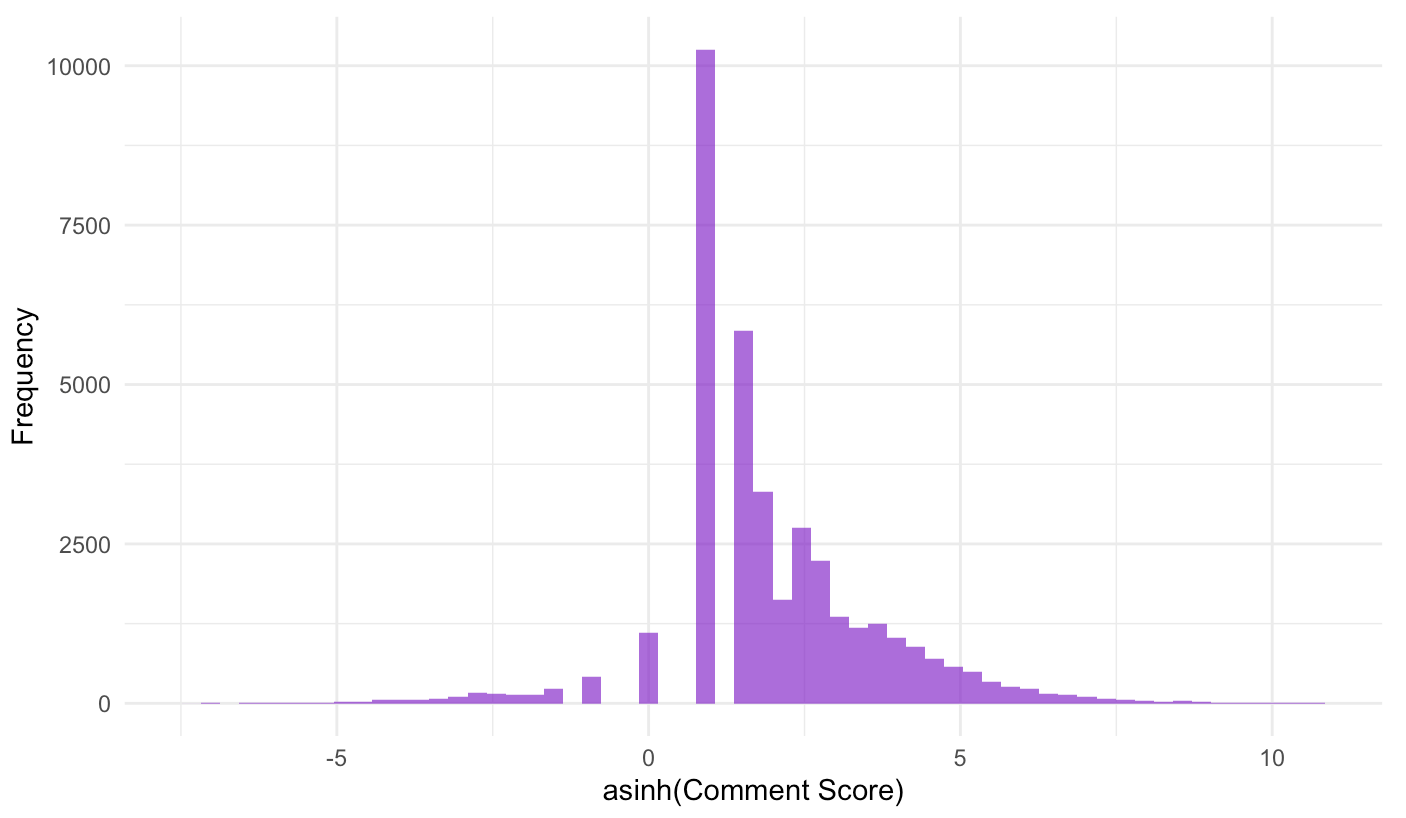
\includegraphics[width=0.7\textwidth]{pictures/ihs_distribution.png}
    \caption{Distribution of Comment Score after applying the IHS transformation.}
    \label{fig:ihs-distribution}
\end{figure}

The inverse hyperbolic sine (IHS) function, defined as
\[
    \operatorname{asinh}(x) \;=\; \ln\!\bigl(x + \sqrt{x^2 + 1}\bigr),
\]
is useful for transforming data that can take on negative, zero, or positive values. According to \citet{burbidge1988}, the arcsinh (IHS) transformation behaves similarly to a log transform for large magnitudes but remains well-defined even for negative or zero observations. This makes it attractive for Reddit comment scores, which can span a wide range of negative and positive values due to upvotes and downvotes. \\

\noindent However, upon inspecting the transformed distribution (Figure~\ref{fig:ihs-distribution}), we notice that there are “gaps” or missing bars in certain ranges of the \(\operatorname{asinh}(\text{Comment Score})\) axis. This suggests that our original data do not contain continuous coverage across all possible values, likely because some specific integer comment scores are never observed. Relying on a transformation that highlights these missing points might bias our inferences. Therefore, we opted against a full regression analysis using the IHS approach. Instead, we turn to Shifted Score Models, which better accommodate the discrete nature and irregularities of the comment score distribution

%--------------------------------------------------

\subsection{Approach 2: Shifted Score Models}
In this approach, we shift the original \texttt{Comment Score} by a constant \(c\) (with 
\(c = |\min(\texttt{Comment Score})| + 1\)) so that all observations are strictly positive:
\[
\text{ScoreShifted} = \texttt{Comment Score} + c.
\]
The truncated distribution of Comment Scores (Figure~\ref{fig:comment-score-zoomed}) suggests that the distribution of the shifted scores resembles a gamma distribution. Based on this observation, we fit three models:
\begin{enumerate}
  \item A \textbf{log-linear Multiple Linear Regression (MLR)} model on \(\log(\text{ScoreShifted})\), which is chosen for its interpretability.
  \item A \textbf{Gamma Regression} model with a log link, which is well suited for the gamma-like, 
  right-skewed nature of the data.
  \item A \textbf{Generalized Additive Model (GAM)} with a Gaussian family to capture potential nonlinear relationships.
\end{enumerate}

\noindent We will assess the significance of predictors across these models and compare their overall performance to determine which approach best explains the variation in Comment Score.

\subsubsection{Log-Linear Multiple Linear Regression (MLR)}
First, we fit a log-linear MLR by taking the natural logarithm of the shifted score and using forward stepwise 
selection based on AIC. This model includes \texttt{Sentiment\_Score} (forced into the model) along with other candidate predictors.

\begin{table}[H]
\centering
\small
\begin{tabular}{lccc}
\toprule
\textbf{Predictor} & \textbf{Estimate} & \textbf{p-value} & \textbf{Remarks} \\
\midrule
(Intercept)                     & 6.679e+00 & $<2\times10^{-16}$ & Baseline level \\
Sentiment\_Score                 & 2.357e-05 & 0.9865    & Not significant \\
Is\_Early\_Comment1              & 6.148e-02 & $<2\times10^{-16}$ & Highly significant \\
Subreddit\_Name (books)          & -5.658e-02 & $<2\times10^{-16}$ & Significant negative effect \\
Subreddit\_Name (datascience)    & -5.223e-02 & $<2\times10^{-16}$ & Significant negative effect \\
Subreddit\_Name (FloridaMan)     & -4.080e-02 & $<2\times10^{-16}$ & Significant negative effect \\
Subreddit\_Name (gaming)         & -4.659e-02 & $<2\times10^{-16}$ & Significant negative effect \\
Subreddit\_Name (Health)         & -3.987e-02 & $<2\times10^{-16}$ & Significant negative effect \\
Subreddit\_Name (movies)         & -4.715e-02 & $<2\times10^{-16}$ & Significant negative effect \\
Subreddit\_Name (Showerthoughts) & -3.406e-02 & $<2\times10^{-16}$ & Significant negative effect \\
Subreddit\_Name (technology)     & -3.742e-02 & $<2\times10^{-16}$ & Significant negative effect \\
Subreddit\_Name (unpopularopinion)& -6.588e-02 & $<2\times10^{-16}$ & Significant negative effect \\
Comment\_Day1                    & -3.084e-02 & $<2\times10^{-16}$ & Significant \\
Comment\_Day4                    & 1.505e-02  & 4.48e-06  & Significant \\
Comment\_Day6                    & 6.070e-03  & 0.005491  & Significant \\
Comment\_Hour10                  & 1.481e-02  & 0.016171  & Significant \\
Comment\_Hour11                  & 4.322e-02  & 4.01e-14  & Highly significant \\
Comment\_Hour12                  & 3.605e-02  & 6.28e-13  & Highly significant \\
Comment\_Hour13                  & 1.395e-02  & 0.001805  & Significant \\
Comment\_Hour14                  & 1.745e-02  & 2.69e-05  & Significant \\
Comment\_Hour15                  & 7.955e-03  & 0.041566  & Significant \\
Comment\_Hour16                  & 1.129e-02  & 0.003557  & Significant \\
Comment\_Hour20                  & 8.401e-03  & 0.030419  & Significant \\
Comment\_Hour22                  & 9.236e-03  & 0.020039  & Significant \\
Parent\_Score                    & 6.311e-07  & $<2\times10^{-16}$ & Highly significant \\
User\_Karma                      & 3.100e-08  & 4.77e-12  & Highly significant \\
Text\_Length                     & 7.568e-06  & 0.008205  & Significant \\
Contains\_Profanity1             & 6.777e-03  & 0.000711  & Significant \\
Contains\_Question1              & 4.400e-03  & 0.002645  & Significant \\
Account\_Age\_days               & 1.155e-06  & 0.005183  & Significant \\
\bottomrule
\end{tabular}

\bigskip
\noindent Adjusted \(R^2\) = 0.0565, F-statistic = 49.1 on 47 and 37709 DF

\caption{Log-linear MLR: Summary of significant predictors}
\label{tab:mlr_results}
\end{table}

\begin{figure}[H]
    \centering
    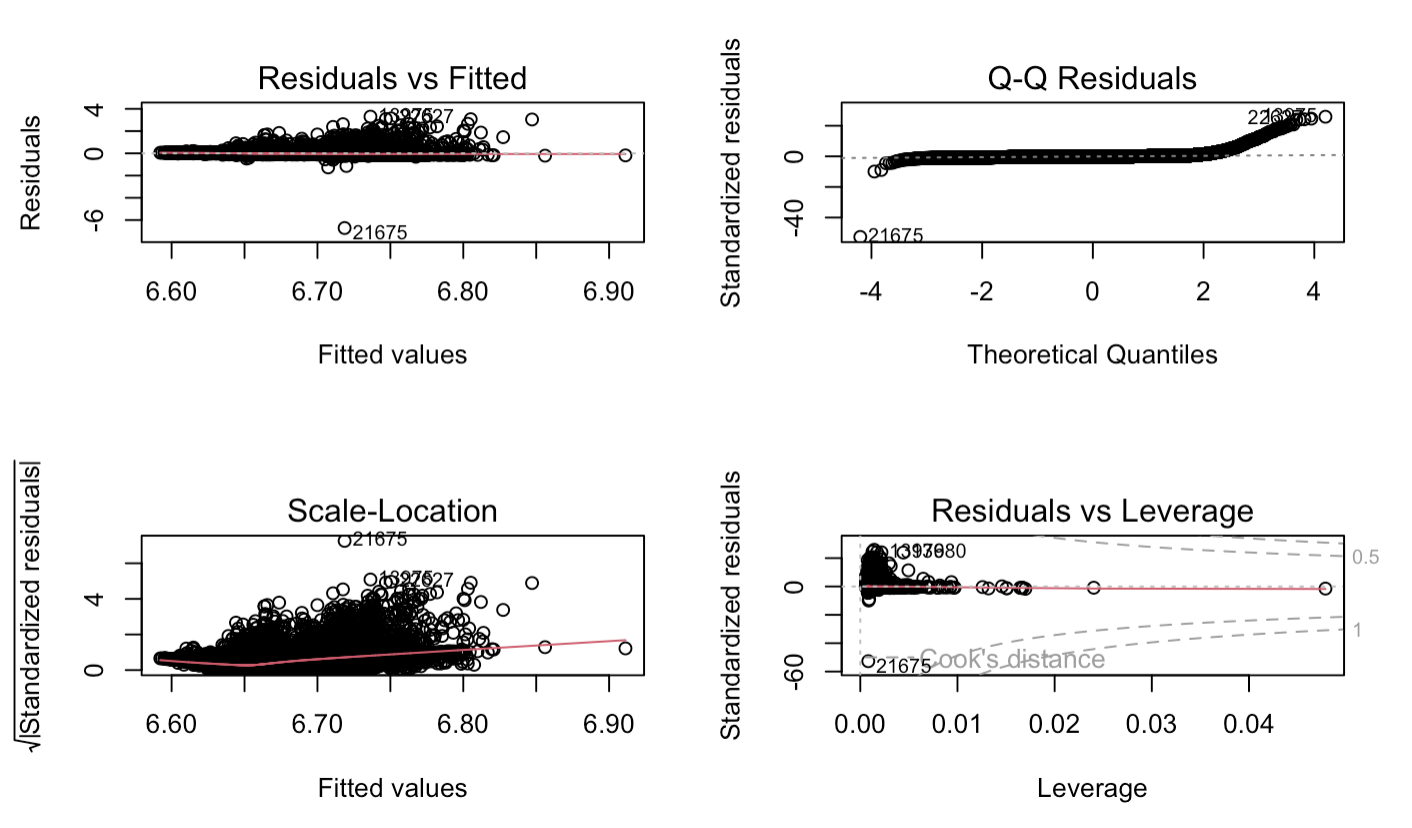
\includegraphics[width=0.7\textwidth]{pictures/log_mlr_plots.png}
    \caption{Diagnostic plots for the log-linear MLR model}
    \label{fig:log_mlr_plots}
\end{figure}

\noindent The stepwise AIC selection process reveals that \texttt{Sentiment\_Score} is not selected as a significant predictor unless explicitly forced into the model; even when included, it remains non-significant (p-value \(\approx 0.9865\)). In contrast, predictors such as \texttt{Is\_Early\_Comment} and several levels of \texttt{Subreddit\_Name}, \texttt{Comment\_Hour}, and \texttt{Comment\_Day} consistently emerge as statistically significant, though their estimated coefficients are relatively small. \\

\noindent The diagnostic plots (Figure~\ref{fig:log_mlr_plots}) reveal that while the residuals tend to cluster around zero, they are not symmetrically distributed: a notable number of residuals are positive, and the distribution exhibits a heavy upper tail. Moreover, the scale-location plot shows that the spread of residuals increases with higher fitted values, indicating heteroskedasticity. These observations suggest that, although some predictors are statistically significant, the model's overall fit is modest (Adjusted \(R^2 \approx 0.0565\)), and there are issues such as non-normality of residuals and non-constant variance that might affect the reliability of inference.

\subsubsection{Gamma Regression with Log Link}
Secondly, given the gamma-like shape of the shifted score distribution, we fit a Gamma regression model with a log link using forward stepwise AIC selection. This model also forces \texttt{Sentiment\_Score} into the model.

\begin{table}[H]
\centering
\small
\begin{tabular}{lccc}
\toprule
\textbf{Predictor} & \textbf{Estimate} & \textbf{p-value} & \textbf{Remarks} \\
\midrule
(Intercept)                     & 6.694e+00 & $<2\times10^{-16}$ & Baseline level \\
Sentiment\_Score                & 5.842e-03 & 0.12074           & Not significant \\
Is\_Early\_Comment1             & 1.068e-01 & $<2\times10^{-16}$ & Highly significant \\
Parent\_Score                   & 2.255e-06 & $<2\times10^{-16}$ & Highly significant \\
Comment\_Hour11                 & 1.252e-01 & $7.45\times10^{-16}$ & Significant \\
Comment\_Hour12                 & 9.531e-02 & $2.53\times10^{-12}$ & Significant \\
Comment\_Hour13                 & 2.440e-02 & 0.04447           & Significant \\
Comment\_Hour14                 & 3.200e-02 & 0.00457           & Significant \\
Comment\_Hour16                 & 2.068e-02 & 0.04926           & Significant \\
Comment\_Hour20                 & 2.641e-02 & 0.01224           & Significant \\
Comment\_Hour22                 & 2.319e-02 & 0.03158           & Significant \\
Subreddit\_Name (books)         & -1.042e-01 & $<2\times10^{-16}$ & Significant negative effect \\
Subreddit\_Name (datascience)   & -9.302e-02 & $<2\times10^{-16}$ & Significant negative effect \\
Subreddit\_Name (FloridaMan)    & -7.714e-02 & 2.70e-09         & Significant negative effect \\
Subreddit\_Name (gaming)        & -8.150e-02 & $<2\times10^{-16}$ & Significant negative effect \\
Subreddit\_Name (Health)        & -7.760e-02 & 2.35e-11         & Significant negative effect \\
Subreddit\_Name (movies)        & -9.312e-02 & $<2\times10^{-16}$ & Significant negative effect \\
Subreddit\_Name (Showerthoughts)& -6.983e-02 & 2.75e-11         & Significant negative effect \\
Subreddit\_Name (technology)    & -7.829e-02 & $<2\times10^{-16}$ & Significant negative effect \\
Subreddit\_Name (unpopularopinion)& -1.118e-01 & $<2\times10^{-16}$ & Significant negative effect \\
Comment\_Day1                   & -5.346e-02 & 8.18e-12         & Significant \\
Comment\_Day4                   & 2.821e-02  & 0.00155          & Significant \\
User\_Karma                     & 6.901e-08  & 1.47e-08         & Highly significant \\
Contains\_Profanity1            & 1.579e-02  & 0.00321          & Significant \\
Account\_Age\_days              & 3.138e-06  & 0.00518          & Significant \\
Contains\_Question1             & 1.047e-02  & 0.00518          & Significant \\
\bottomrule
\end{tabular}

\bigskip
\noindent Dispersion parameter for Gamma family: 0.1201041 \\ Null deviance: 1196.3 on 37756 degrees of freedom \\ Residual deviance: 1035.2 on 37710 degrees of freedom
\caption{Gamma Regression: Summary of significant predictors}
\label{tab:gamma_results}
\end{table}

\begin{figure}[H]
    \centering
    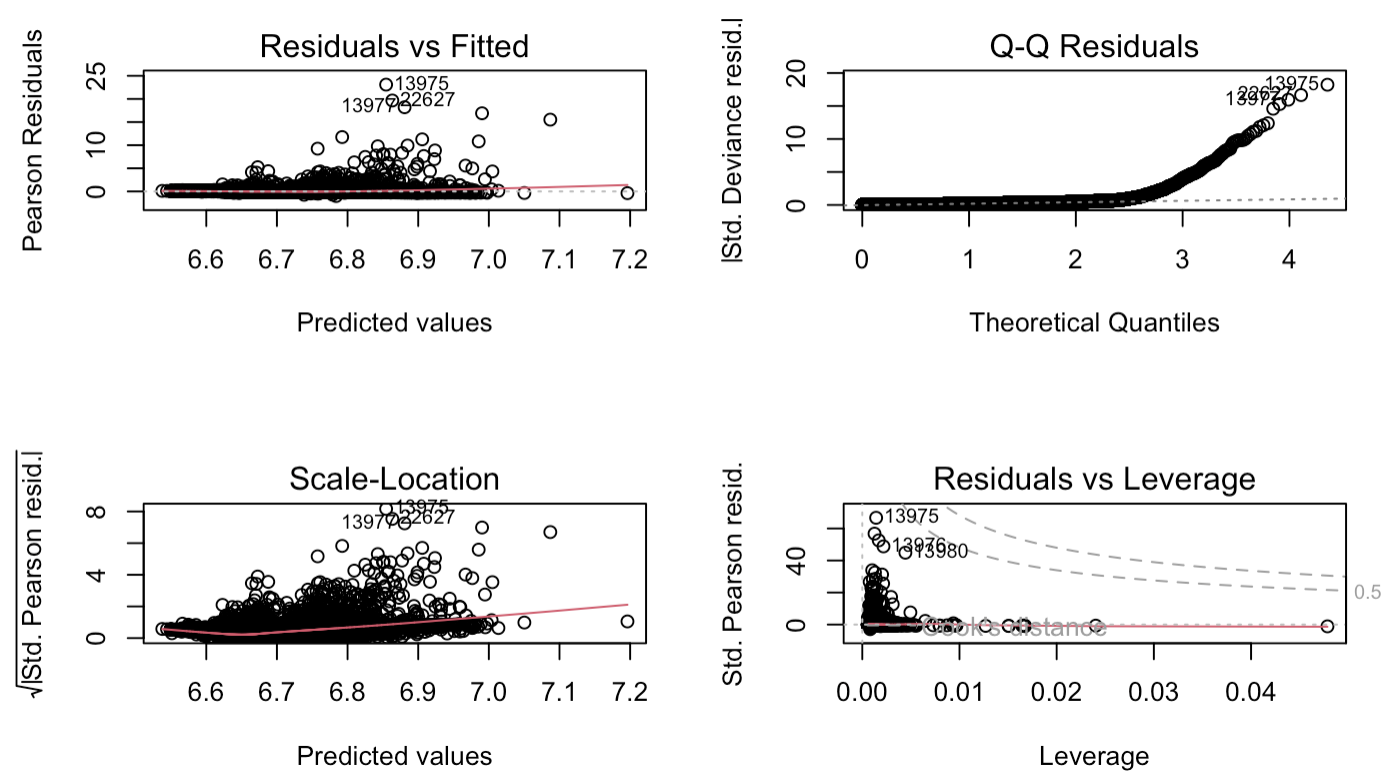
\includegraphics[width=0.7\textwidth]{pictures/gamma_plots.png}
    \caption{Diagnostic plots for the Gamma regression model with a log link.}
    \label{fig:gamma_plots}
\end{figure}

\noindent The Gamma regression model shows a pattern of significant predictors that is largely consistent with the log-linear MLR model. In both models, predictors such as \texttt{Is\_Early\_Comment}, \texttt{Parent\_Score}, and various levels of \texttt{Subreddit\_Name}, and \texttt{Comment\_Hour} are highly significant, while \texttt{Sentiment\_Score} remains non-significant. The Gamma model reports a null deviance of 1196.3 and a residual deviance of 1035.2, suggesting a modest reduction in deviance relative to the null model, though a substantial portion of variability remains unexplained. \\

\noindent Additionally, the diagnostic plots for the Gamma model (Figure~\ref{fig:gamma_plots}) exhibit trends similar to those observed in the log-linear MLR model: the scale-location plot indicates an increasing spread of residuals at higher fitted values, and the Q-Q plot reveals deviations from normality, particularly with a heavy upper tail. These similarities suggest that both models capture comparable underlying dynamics in the data, even though the Gamma model is more appropriate for the positive, skewed distribution of the shifted comment scores.

\subsubsection{Generalized Additive Model (GAM)}
Lastly, we fit a GAM to capture potential nonlinear effects. Smooth functions are applied to continuous predictors such as \texttt{User\_Karma}, \texttt{Word\_Count}, \texttt{Account\_Age\_days}, \texttt{Text\_Length}, \texttt{Parent\_Score}, and \texttt{Sentiment\_Score}.

\begin{table}[H]
\centering
\small
\begin{tabular}{lccc}
\toprule
\textbf{Predictor / Smooth Term} & \textbf{edf / Estimate} & \textbf{p-value} & \textbf{Remarks} \\
\midrule
\multicolumn{4}{l}{\textbf{Smooth Terms:}} \\
s(User\_Karma)       & 7.209       & $<2\times10^{-16}$ & Strong nonlinear effect \\
s(Account\_Age\_days) & 6.271       & 0.0159             & Significant nonlinearity \\
s(Parent\_Score)     & 8.645       & $<2\times10^{-16}$ & Strong nonlinear effect \\
s(Sentiment\_Score)  & 1.150       & 0.0851             & Borderline, not significant \\
\midrule
\multicolumn{4}{l}{\textbf{Parametric Terms:}} \\
(Intercept)                     & 8.173e+02 & $<2\times10^{-16}$ & Baseline level \\
Is\_Early\_Comment1              & 9.279e+01  & $<2\times10^{-16}$ & Highly significant \\
Subreddit\_Name (books)          & -7.031e+01 & $<2\times10^{-16}$ & Significant negative effect \\
Subreddit\_Name (datascience)    & -5.655e+01 & $<2\times10^{-16}$ & Significant negative effect \\
Subreddit\_Name (FloridaMan)     & -5.321e+01 & 2.70e-09 & Significant negative effect \\
Subreddit\_Name (gaming)         & -7.152e+01 & $<2\times10^{-16}$ & Significant negative effect \\
Subreddit\_Name (Health)         & -5.055e+01 & 2.35e-11 & Significant negative effect \\
Subreddit\_Name (movies)         & -7.348e+01 & $<2\times10^{-16}$ & Significant negative effect \\
Subreddit\_Name (Showerthoughts) & -5.734e+01 & 2.75e-11 & Significant negative effect \\
Subreddit\_Name (technology)     & -6.327e+01 & $<2\times10^{-16}$ & Significant negative effect \\
Subreddit\_Name (unpopularopinion)& -7.757e+01 & $<2\times10^{-16}$ & Significant negative effect \\
Comment\_Day1                   & -3.409e+01 & 7.40e-06 & Significant \\
Comment\_Day4                   & 1.850e+01  & 0.03349 & Significant \\
Comment\_Day6                   & 1.093e+01  & 0.06374 & Borderline \\
Comment\_Hour10                 & 3.661e+01  & 0.02305 & Significant \\
Comment\_Hour11                 & 1.247e+02  & $<2\times10^{-16}$ & Highly significant \\
Comment\_Hour12                 & 8.540e+01  & 7.88e-11 & Highly significant \\
Comment\_Hour14                 & 2.834e+01  & 0.00917 & Significant \\
Comment\_Hour20                 & 2.572e+01  & 0.01145 & Significant \\
Comment\_Hour22                 & 2.174e+01  & 0.03671 & Significant \\
Contains\_Profanity1            & 1.059e+01  & 0.04414 & Significant \\
\bottomrule
\end{tabular}

\bigskip
\noindent R-sq.(adj) = 0.0387, Deviance Explained = 4.05\%\\
\caption{GAM: Summary of significant Smooth and Parametric Terms}
\label{tab:gam_results}
\end{table}


\begin{figure}[H]
    \centering
    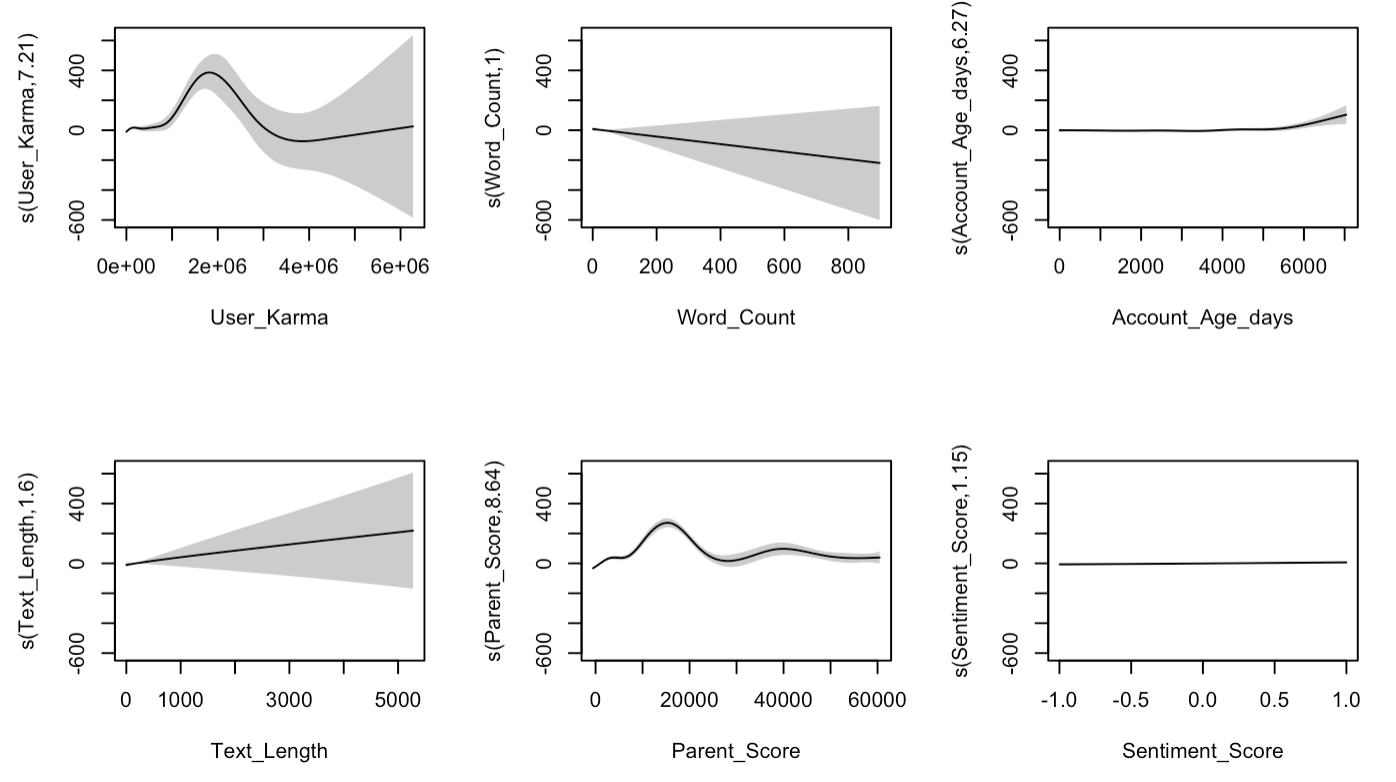
\includegraphics[width=0.7\textwidth]{pictures/gam_plot_1.png}
    \caption{GAM Smooth Terms' Plots}
    \label{fig:gam_smooth_plots}
\end{figure}

\begin{figure}[H]
    \centering
    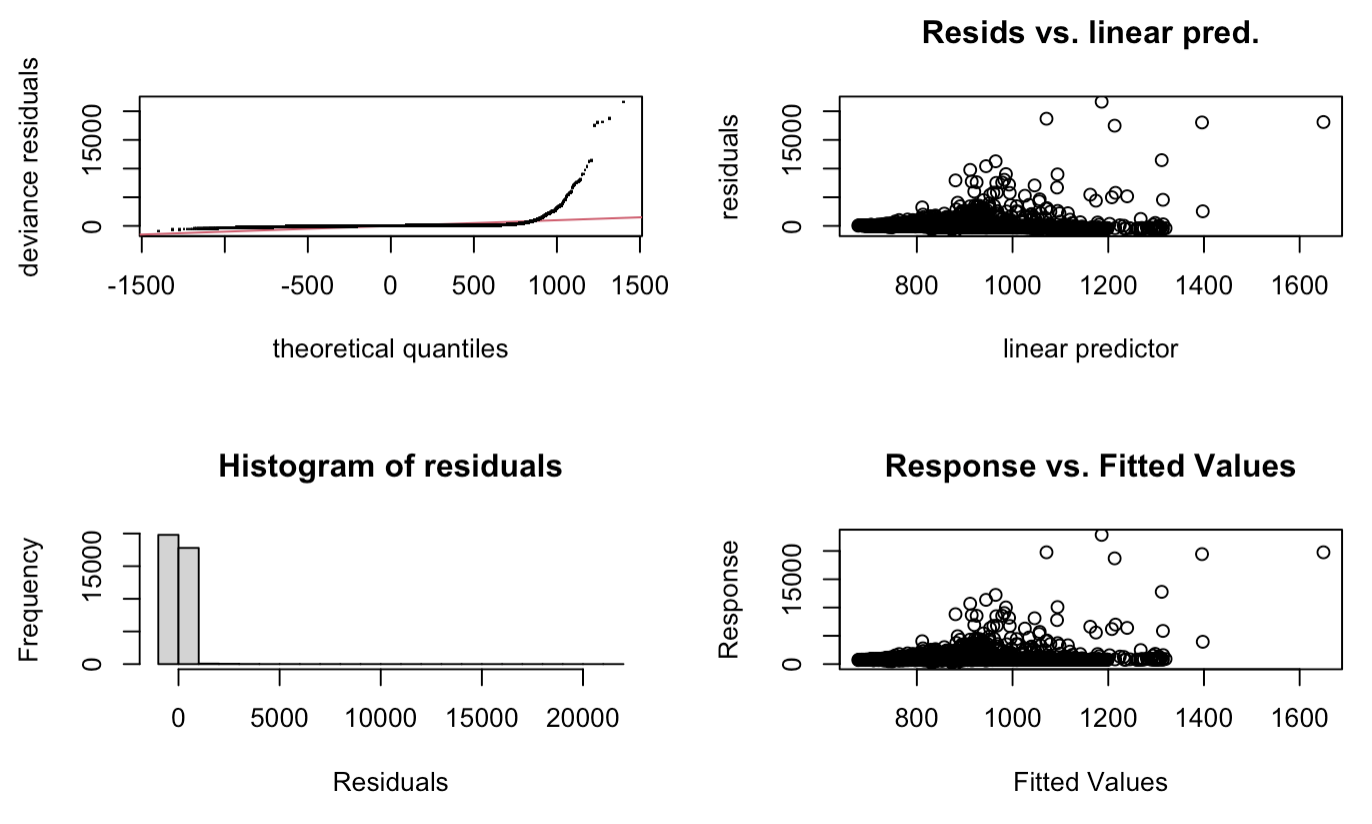
\includegraphics[width=0.7\textwidth]{pictures/gam_plot_2.png}
    \caption{GAM Diagnostic Plots}
    \label{fig:gam_diag_plots}
\end{figure}

\noindent This GAM model, which includes both smooth and parametric terms, has an adjusted \(R^2 \approx 0.0387\) and explains about 4.05\% of the deviance, indicating a relatively low level of overall fit—similar to the modest performance seen in the log-linear MLR and Gamma models. As in those models, \texttt{Is\_Early\_Comment} and certain \texttt{Subreddit\_Name} levels remain significant, whereas \texttt{Sentiment\_Score} is not significant even when modeled nonlinearly. \\

\noindent From the smooth plots in Figure~\ref{fig:gam_smooth_plots}, we see that \texttt{User\_Karma} and \texttt{Parent\_Score} display strong nonlinear effects, suggesting more complex relationships with \texttt{Comment\_Score\_shift} than a simple linear model could capture. Meanwhile, smooth terms like \texttt{Word\_Count} and \texttt{Text\_Length} are not significant, indicating no pronounced nonlinearity for those predictors in this model.\\

\noindent The diagnostic plots in Figure~\ref{fig:gam_diag_plots} echo patterns from the other two approaches: the Q-Q plot suggests the residuals deviate from normality, and the residuals vs.\ fitted values indicate a non-constant spread. Hence, although the GAM can capture some nonlinear trends (notably for \texttt{User\_Karma} and \texttt{Parent\_Score}), it does not substantially improve the overall explanatory power compared to the log-linear MLR or the Gamma regression. 

%--------------------------------------------------

\section{Conclusion and Recommendations}

Despite exploring several modeling approaches, none of the models achieved a robust overall fit, as reflected by the relatively low adjusted \(R^2\) values. This indicates that a substantial portion of the variability in the shifted comment scores remains unexplained. Several factors may contribute to this outcome, including the skewing effect of extreme positive values (i.e., viral comments), the relative rarity of negative comment scores, and unmeasured influences, such as the specific textual content of comments, that our current predictors fail to capture. Among the models evaluated, the log-linear Multiple Linear Regression (MLR) offers the best balance; it is straightforward and interpretable while still explaining a modest fraction of the variance in comment popularity. \\

\noindent The central hypothesis of our study was that the sentiment of a comment would significantly impact its popularity. However, across all three models, the variable \texttt{Sentiment\_Score} consistently emerged as non-significant. In contrast, various metadata features proved to be more influential. For instance, \texttt{Is\_Early\_Comment} was highly significant, indicating that early posting tends to lead to higher engagement. Moreover, several levels of \texttt{Subreddit\_Name} were significant; specific subreddits such as \texttt{books}, \texttt{datascience}, and \texttt{unpopularopinion} systematically recorded lower scores relative to the baseline. Time-related predictors, including distinct \texttt{Comment\_Day} and \texttt{Comment\_Hour} variables, also demonstrated significance, suggesting that both the day and hour of posting can influence comment popularity. Overall, these findings imply that metadata features play a more crucial role than sentiment in predicting Reddit comment popularity. \\

\noindent Future research should leverage state-of-the-art natural language processing methods to better capture the nuanced sentiment and context of Reddit comments. Instead of traditional sentiment analysis, transformer-based models such as RoBERTa could be employed to identify subtle language cues, including sarcasm and context-dependent sentiment, which standard approaches often miss. Additionally, topic modeling techniques like BERTopic could reveal specific themes or clusters within the comment data, providing more granular insights into what drives engagement across various subreddits. \\

\noindent Furthermore, incorporating user-level data through hierarchical Bayesian models could further enhance our understanding by accounting for the nested structure of Reddit interactions, such as comments within posts and subreddits. Complementing these approaches with social network analysis could quantify user influence and reveal network effects that impact comment popularity. By integrating these advanced methodologies and richer, multi-level data, future research could yield models with higher explanatory power and offer deeper insights into the dynamics of online discourse.

\clearpage
\bibliographystyle{plainnat}
\bibliography{references}

\end{document}
